\documentclass[a4paper,11pt]{article}

% ------------ Renew commands to have correct counting in enumerate env

\renewcommand{\theenumi}{\thesubsection.\arabic{enumi}}
\renewcommand{\labelenumii}{\theenumii}
\renewcommand{\theenumii}{\theenumi.\arabic{enumii}.}

% ------------ Import Requirements Elicitation for Referencing
\usepackage{xr}
\externaldocument{../Requirements/Requirements_Elicitation}

\usepackage[utf8]{inputenc}
\usepackage[top=3cm, bottom=3cm, left=3cm, right=3cm]{geometry}
\usepackage[none]{hyphenat}
\usepackage{xcolor,colortbl}
\definecolor{Gray}{rgb}{0.9,0.9,0.9}
\usepackage{graphicx}

% mention: validate performance requirement (5sec) after implement process
% risks? resouces (people..)?
% reference the diagram from overview in requirements in design document component diagram again (and then specify to only describe the server modules here)
% Example client (Technology choices) couple off clearly
% !! Reason about all stuff in the document and reference the requirements

% ------------ Title section
\title{
\vspace{-8cm}
\begin{flushleft}
    \vspace{10cm}
    \normalfont \normalsize
    %\Huge Bachelor/Master Thesis Project \\
    \vspace{-1.3cm}
\end{flushleft}
\vspace{3cm}
\begin{flushleft}
    \huge Face Recognition System \\
    \LARGE  Design Document\\
\end{flushleft}
\null
\vfill
\begin{minipage}{\textwidth}
\begin{flushleft} \large
\emph{Authors:} Walid Balegh, Jakob Heyder, Sarpreet Singh Buttar, Henry \hspace{45pt} Pap and Oscar Maris \\ % Author
%\emph{Supervisor:} Name of your supervisor\\ % Supervisor
%\emph{Examiner:} Dr.~Mark \textsc{Brown}\\ % Examiner (course manager)
\emph{Semester:} VT 2017\\ %
%\emph{Subject:} Computer Science\\ % Subject area
\end{flushleft}
\end{minipage}
}

\date{}

\begin{document}

\maketitle

\newpage

\tableofcontents

\newpage


\section{Introduction}
The FRS (face recognition system) design document is intended to be the groundwork of how the software should be built.
%still working on the indroduction don't want it to sound too much like purpose

\subsection{Purpose}
The design documentation of the FRS is intended to create a mutual understanding of the software's functionality and contents. This document should contain all necessary information to start development of the face recognition system. This includes all known technologies, pitfalls and the architecture for the FRS as a whole.


\subsection{Priorities}
%Priorities
%	- Security - Encryption and Authentication , sensible data
%	- Portability/Integration \& Usability - clear defined API
%	- Reliability

Security: As we are dealing with users private information it imperative that the system is both secure and has limited access for both users and administrators. The primary methods to achieve this will be: The use of HTTPS SSL/TLS and both admin and user authentication.

Reliability: When the user requests a PN from the server there needs to be a certain guarantee that that the PN returned matches the image provided.

Portability: Creating a application that uses the FRS should be both possible and simple for a variety of devices and there operating systems. It should also be reliable on a number of different operating systems that come with these devices.

Usability: The system should have clear defined methods and structure that will not be misinterpreted. The user application developed, should also be user friendly with the user interface having clear definitions.

\subsection{Overview}
This design document is for the face recognition software. The FRS purpose is to provide a PN (swedish Personal Number) using a comparison of a user provided image of a person's face. There should also be authentication to both users and administrators in place. Administrators should also have access to a list of the PNs from the database. Administrators are also able to add, edit and delete entries from the database.
Additionally to the FRS a user application will also be developed to present the user functionality of the system. Said application should include the ability to authenticate the user and request PNs using images.

\section{Major Design Issues} \label{Major_Design_Issues}
In this section all major design issues and decisions will be discussed. Rational and alternatives will be presented and the detail of evaluating the alternatives depends on the trade off the decision has.

\subsection{Architectural Design} 
As desired from the customer the system will have a Client-Server structure. Where the in section \ref{ReqDefinitions} of the Requirements Elicitation defined UAM and AAM are the client modules and the URM and ARM are the server modules. Further we may reference URM or ARM as Server and UAM and AAM as Client. It is important to note that as defined in the requirements Req. Doc. \ref{ReqSystemInterfaces} our developed product is only the Server with a clear API and the Client application we talk about is the desired example client to show how integration and usage could be done.
The architecture of the server is defined in detail in \ref{Architecture}.

\subsection{Languages \& Frameworks}
\subsubsection{Server-side}
As choice of programming language we choose the \textbf{Java programming language}. It is one of the most widely used ones on the server side. Especially the  in \ref{ReqProductFunctions} of the Requirements Elicitation defined REST functionality is supported by various frameworks with large communities. Rationals which led to the choice are listed below.
\begin{itemize}
\item Great flexibility \& portability due to platform independence with the JVM.
\item Scalable solution based on proven enterprise solutions
\item High productivity because of existing frameworks and solutions
\item Good support by a large community of developers
\end{itemize}

The Spring Framework will be used on the server side of the system.
More detailed the Spring Web, Security, Data and Boot modules. This modules support the 
The Spring Framework allows fast, enterprise scale development of applications by providing features for security, RESTful applications and Data Management and thus is the perfect fit for the requirements defined in the Requirements Elicitation \ref{ReqProductFunctions} and \ref{ReqConstraints} such as authentication, encryption and REST functionality. The Rationals for using the different modules are listed more detailed below.
\begin{itemize}
\item Great Portability and Integration - it is supported by various cloud providers to make deployment and continuous development possible.
\item Spring Boot provides an embedded application server which allows fast and easy setup of an application.
\item Configurability - Spring is easily set up and gives good default solutions but also provides the possibility to configure the details to the application needs
\item The Spring framework provides RESTful support which is asked for from the customer and fills the application needs.
\item Spring Data provides a convenient way to implement CRUD functionality for accessing and modifying data. It supports various Database technologies such as JPA and generates boilerplate code at run time which reduces developing costs.
\item Spring Security provides enterprise ready security features for authentication and encryption without much setup.
\end{itemize}

\subsubsection{Client-side}
\noindent The client application as defined in \ref{User_Interfaces} of the Requirements Elicitation has to be working on mobile or web browsers. It is therefore suitable to make a web browser interface which is also responsive on mobile. Thus the application will be able to run on iOS, Android, Microsoft phone and WEB. Alternatively it could be developed with one of various Cross Platform Mobile development tools out there. Some of them are listed below.

\begin{itemize}
\item
  \textbf{Xamarin} - which is the most popular choice, a free trail is
  available and it use the language C\#. This will make it more
  structured as C\# is an \emph{OO} language.
\item
  \textbf{Phone Gap} - which is the most well known tool, it is open
  source meaning that it is free. It uses the common web languages to
  create hybrid apps i.e.~HTML, CSS, JavaScript.
\item
  \textbf{appcelerator} - lets developers use JavaScript to build their
  apps, provide mobile testing, it has a GUI to create design (which
  uses common HTML and CSS), and lastly it is free.
\end{itemize}

\noindent There is plenty more but since we only want to show the usage of the API by example as written in the Requirement Elicitation \ref{ReqSystemInterfaces} we will not need a native application. Using common WEB languages to create a browser alternative fulfills the requirements. No requirements constrain the decision among various alternatives for the Web development. Thus this will be discussed in the next section \ref{Technology_choices}

\subsection{Communication Technology}

\subsubsection{Communication}
The Communication will be over IP/TCP to have reliable transport and uses HTTPS on the application layer. This ensures general security by using SSL/TLS and ensures data integrity and privacy by authenticating the application. It provides the encryption and security defined in \ref{ReqConstraints} of the Requirements Elicitation.

\subsection{External Services}

\subsubsection{External Face Recognition API}
One of the core features as defined in \ref{ReqProductFunctions} of the Requirements Elicitation is to match a photo of a face with an existing one to a certain factor of equivalence/similarity. For this purpose as defined in the requirements an external service will be used. Following we compare some of the most known ones. Important aspects are cost factor, usability for the specific needs and security support.
There are some External Face Recognition API out there such as
\begin{itemize}
\item \emph{SkyBiometry: } It is a cloud-based face detection and recognition software which provides a high-precision biometric identification for over 20 years. In addition, it also provide API client libraries in various languages such as Java, C\#, Pyton etc for giving a quick start to the developers. Regarding the usage limits, it has a free subscription which allows 100 methods calls hourly and 5000 monthly. It provide SSL support and its API uses REST interface which means all the API methods are called over the Internet using standard HTTP methods and responses are generated in XML or JSON.
\item \emph{Lambda Labs: } It permits developers to send an image link to their service for the identification. In addition, it also allow to create an album of photos, analyze and compare new images with existing ones. Regarding the usage limits, it has a no free subscription and minimum cost is \$9/month. It does not provide SSL support and its API also uses REST interface and responses are generated in JSON.
\item \emph{OpenFace: } It is a open source web service which provide facial detection technologies. Its API uses REST interface and accept image from the developer and return a JSON response. Currently, it does not support SSL and can only detect up to 80 points on a given image.
\end{itemize}
We have found that \emph{OpenFace} does not provide sufficient functionality as compared to others. Wheres \emph{Lamba Labs} does provide needed functionality but with a cost of \$9/month. In result, \emph{\textbf{SkyBiometry}} is the free and suitable option for our project.

\subsection{Application specific}
Authentication as defined in \ref{ReqConstraints} of the Requirements Elicitation will be done by providing a username and password for registered Users and Admins. The Registration will be exclusive over  a non automated channel by contacting the Customer/Developers to verify a service. The in \ref{ReqConstraints} the Requirements Elicitation mentioned credentials refer further to a user name and password.

\subsection{Data format}
The data will be formatted in standard JSON for communications between the server and the client. The format is human-readable and widely supported. It also supports the requirements of a RESTful application.(Req.Elic. \ref{ReqProductFunctions})

\section{Technology choices} \label{Technology_choices}
In this section we will discuss technology choices which are not constrained by the requirements and thus do not belong directly into the design space defined in \ref{Major_Design_Issues}

\subsection{Client technology}
 In this section we will shortly discuss the technologies used for developing the WEB Client. \textit{It is important to mention that this is not a client in the classical sense as that the browser is the communicating instance and the client only consists of the pages served from a web-server. So it is more only a user interface to access the API.} \\
 We will use responsive design to style our app so it will be desktop, tablet and mobile friendly. For this we will use a CSS framework, all CSS frameworks comes also with a JavaScript framework for design purpose (animation etc.). Further a list of recent CSS frameworks:

\begin{itemize}
\item
  \textbf{Bootstrap} - the most common framework out there, easy to use
  and creates fast design. Great for dynamic designing thanks to its
  grid system. The major drawback is that it will look boring and old.
\item
  \textbf{Material Framework} - Google's own framework, a google look
  alike framework.
\item
  \textbf{Semantic UI} - a fresh framework that has grown quite popular
  in the last couple of years. It uses the JavaScript jQuery framework
  which is easy to use and has great AJAX calls which can be helpful.
\end{itemize}

\noindent This is only a design option and we will go with the Semantic UI because it has a suiting design, and for the use of jQuery. 

\subparagraph{To summarize}\label{to-summarize}
The framework that will be in used for WEB development is Semantic UI
for CSS and jQuery for JavaScript as it comes with Semantic UI.

\subsection{Development Platforms}

\subsubsection{Platform Server}
The Server will run on a cloud platform. This gives several advantages which are listed below. Especially easy setup and management are essential for this project during development and by using Java the components are platform independent which allows later changes during production.
\begin{itemize}
\item Easy to manage and setup - no System administrator needed
\item Allows fast and continuous development and testing
\item Cheap and scalable solution
\end{itemize}

For the development in the cloud, Heroku is among AWS, Microsoft Azure, Google application engine and others a common choice. It supports good conditions for development and support frameworks for features such as database deployment. This gives a convenient way to get the system fastly up and working. Listed are features it provides.
\begin{itemize}
\item Native support for Java and Spring Boot application deployment
\item Addon support for rational Databases (e.g. MYSQL)
\item Github integration for continuous development
\item Free use for small scale applications (development)
\end{itemize}

\subsubsection{Platform Client}
The Client, more specific the in the to be developed UAM will be Web compatible. Since it is written in Javascript for mobile development it runs on iOs, Android and every system supporting modern web browsers.

\subsection{Database}
The database will be MYSQL a rational database.
It is one of the most used rational databases and therefore provides sufficient features, support and scalability for the application. It is also compatible with the used Spring framework and the Heroku cloud platform. It validates data and ensures integrity.




\section{Architecture (Component Diagram)} \label{Architecture}
The subsystems of our system must be reusable and independent from each
other, as that will make it easier to implement and test. The different
subsystems or components are then combined by the application (which is
our system). We define the different components in the component list,
then we explain each of them briefly.

\paragraph{Component list}\label{component-list}

\begin{itemize}
\item
  authenticate
\item
  admin
\item
  user
\item
  face
\item
  database
\item
  storage
\item
  skyBiometry
\item
  imgur
\item
  MySQL
\end{itemize}

\paragraph{Component details}\label{component-details}

Now we will discuss why we need the different components, how they will
be used and what they will require.

\subparagraph{1. authentication}\label{authentication}

The authentication component is required for security and divides the
system based on whether the connected client is an user or an admin \ref{2.1.6 Security constraints}. The
required interface for authentication is the database component, the
provided interface is a login functionality that returns an integer 0 -
no match, 1 - user and 2 - admin and a check which checks if current
client is logged in (user or admin).

\subparagraph{2. admin}\label{admin}

The admin component is a core component that will hold all the admin
responsibilities which is management of client users (faces). The
required interface is the face, storage and database component. The
provided interface is the CRUD methods check \ref{3.3 Admin Repository Module} at line 3.3.4.

\begin{itemize}
\item
  CREATE : create a new user
\item
  READ : get the user information by id or all.
\item
  UPDATE : updates an existing user by id
\item
  DELETE : removes an existing user by id
\end{itemize}

\subparagraph{4. user}\label{user}

The user component is also a core component that will be responsible of
getting a Swedish social security number based on a image check \ref{User Repository Module} in the requirements elicitation. The required
interface is the face, database and the provided interface is
``\emph{uploading a picture}''. 

\subparagraph{4. face}\label{face}

The face is the main component of this system (FRS), this needs to be as
independent as possible in order of our system to be adaptive to changes
(i.e.~face-recognition algorithm may be replaced in the future for a
better one). The required interface that is needed is skyBiometry (the
face-recognition api) and the provided interface is CRUD methods \ref{Admin Repository Module}, which
allows admins to manage client faces as well as letting user component
get a PN based on a picture, see \ref{User Repository Module}.

\subparagraph{5. database}\label{database}

The database or actually database-access component is the component that
will directly talk with the remote database. The required interface is a
MYSQL-database since it is flexible and easy to use, but can easily be replaced. The provided is CRUD methods as well as a login method. This is a nessesary component check \ref{System Interfaces} in the requirements elicitation: ``\emph{Personal number database}'' will also hold information of login-users.

\subparagraph{6. storage}\label{storage}

The storage component is the component that will save the client-face
picture to the storage, see \ref{System Interfaces}, the ``\emph{Image Database}'' now we will use imgur.com api to store pictures
as space is an issue but in future this can be changed into storing
images directly in our server. The required interface is imgur.com-api
and the provided interface is upload picture.

\subparagraph{7. skyBiometry}\label{skybiometry}

The face-recognition algorithm api, we will use skyBiometry as discussed
earlier.

\subparagraph{8. imgur}\label{imgur}

The imgur or imgur.com-api will be used by our storage component.

\subparagraph{9. MySQL}\label{mysql}

MySQL is the database type we will use by the database-access component.

\paragraph{Architecture Pattern}\label{architecture-pattern}

We already mentioned that the system will have client-server structure in \ref{2.1 Architectural Design}, but now we focus only on the server part as it is our only implementation part, clients then can connect and use our service the server provide.
We want good reusability, good cohesion, low coupling, abstraction, security and
portability all this because components should be easily changeable,
independent so development can be as well and portable so the system can
easily be changed to other servers (in the future). Our system is a
layer type where the application (which will act as the glue code) will
use authentication, admin and user component and these will use the
others. See the component diagram to clearly see why it will be a
layered system. The patterns that meets our required types
i.e.~cohesion, coupling, abstraction and portability is:

\begin{itemize}
\item
  Multi-layers
\item
  Service-oriented
\end{itemize}

The Service-oriented pattern focus on the communication between the
different web-services, in our case is with MySQL database, imgur.com
api and skyBiometry. This will use standard communication HTTP which in
the core basics is XML as the pattern says it should be (open
standards). This is a very good pattern to follow when it comes to our
remote components.

The Multi-layers pattern focus on how the communication should be,
i.e.~layer can only speak with the layer below it, in our case the
different components can only speak with the required components and not
the other way around (see component diagram to better understand). This
is also a very good pattern for our system that focuses on the structure
of the system.

\subparagraph{Conclusion}\label{conclusion}

We will use a combined pattern, Multi-layers pattern (for developed
component) and Service-oriented pattern (for communication with remote
components).

\newpage

\subsubsection{Diagrams}\label{diagrams}

\paragraph{Component Diagram}\label{component-diagram}

\begin{figure}[ht!]
	\centering
	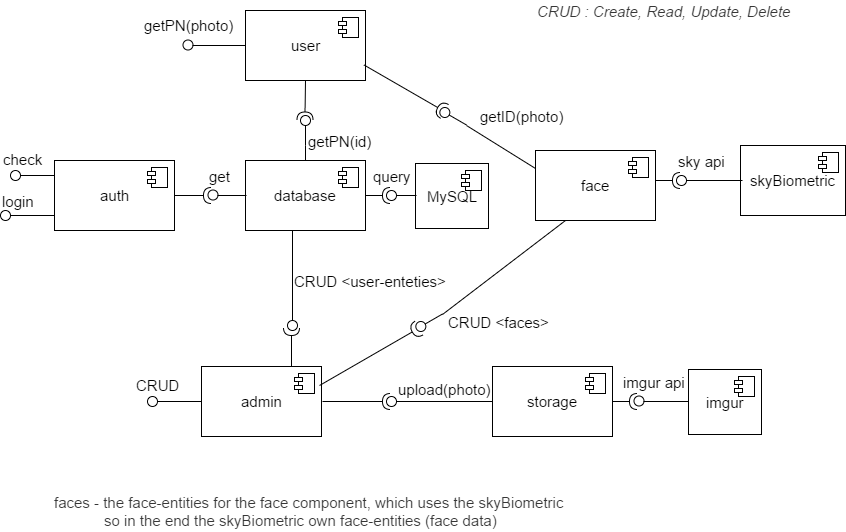
\includegraphics[width=150mm]{Architecture/ComponentDiagram.png}
	\caption{ComponentDiagram}
\end{figure}

\paragraph{Deployment Diagram}\label{deployment-diagram}

\begin{figure}[ht!]
	\centering
	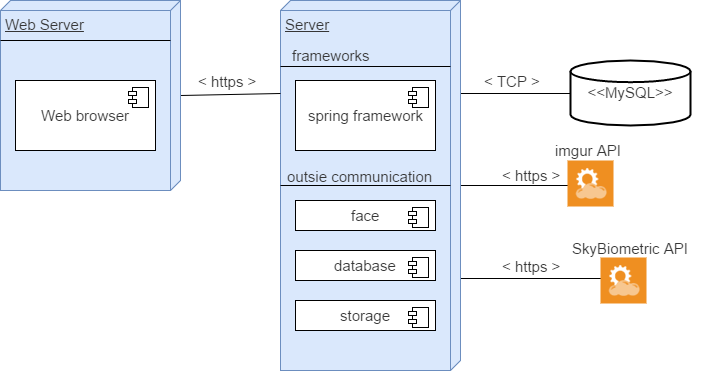
\includegraphics[width=150mm]{Architecture/DeploymentDiagram.png}
	\caption{DeploymentDiagram}
\end{figure}
\newpage

\section{Components - Static modeling (Class Diagrams)}


\section{Use cases - Behavioral modeling (Sequence Diagrams)}

\begin{figure}[ht!]
	\centering
	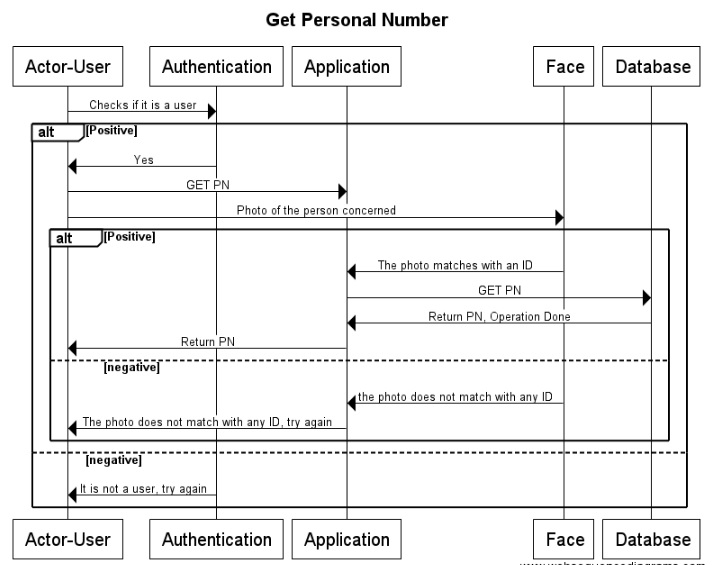
\includegraphics[width=150mm]{SequenceDiagrams/GetPN.jpg}
	\caption{Sequence diagram referred to "5.2 UAM: GET Personal Number" in the requirement document. \label{1}}
\end{figure}

\begin{figure}[ht!]
	\centering
	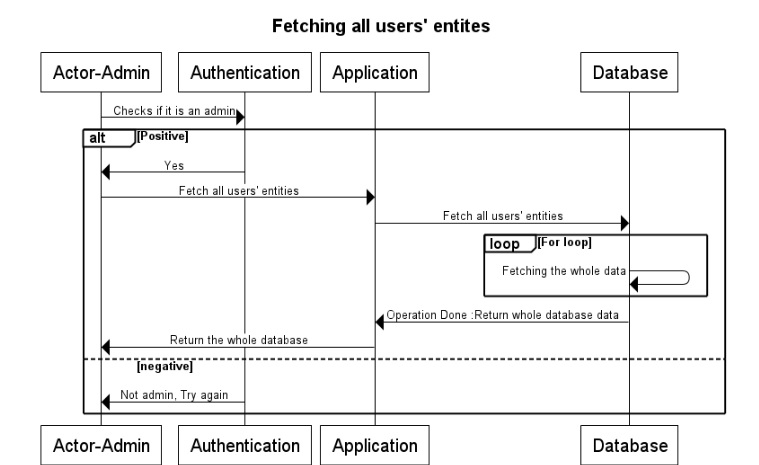
\includegraphics[width=150mm]{SequenceDiagrams/FetchAllUsers.jpg}
	\caption{Sequence diagram referred to "5.3 ARM: Get List of User-Entities" in the requirement document. \label{2}}
\end{figure}
\begin{figure}[ht!]
	\centering
	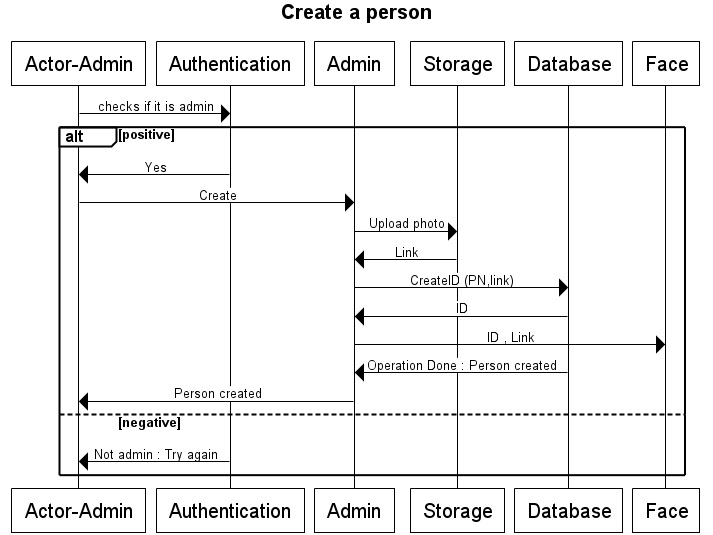
\includegraphics[width=150mm]{SequenceDiagrams/Create.jpg}
	\caption{Sequence diagram referred to "5.4 ARM: Add an User-Entity" in the requirement document. \label{3}}
\end{figure}

\begin{figure}[ht!]
	\centering
	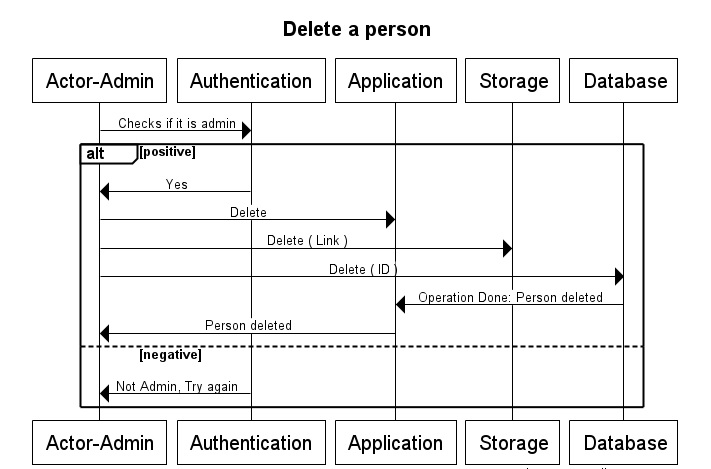
\includegraphics[width=150mm]{SequenceDiagrams/Delete.jpg}
	\caption{Sequence diagram referred to "5.5 ARM: Delete an User-Entity" in the requirement document. \label{4}}
\end{figure}

\begin{figure}[ht!]
	\centering
	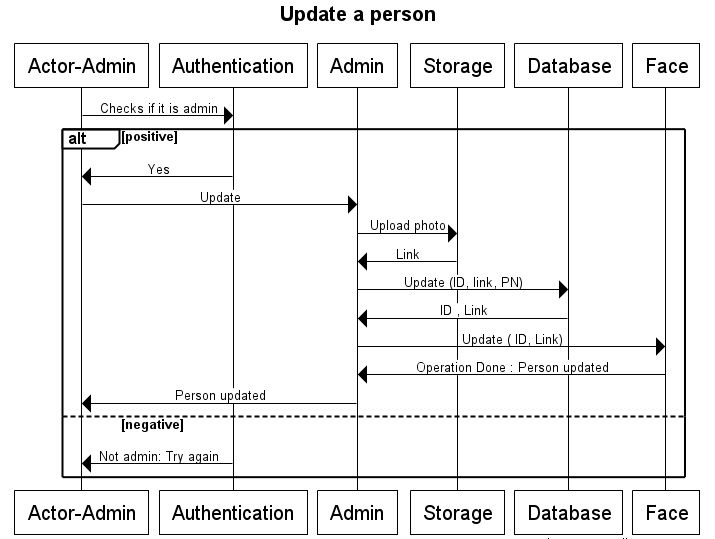
\includegraphics[width=150mm]{SequenceDiagrams/Update.jpg}
	\caption{Sequence diagram referred to "5.6 ARM: Update User-Entity" in the requirement document. \label{5}}
\end{figure}

\begin{figure}[ht!]
	\centering
	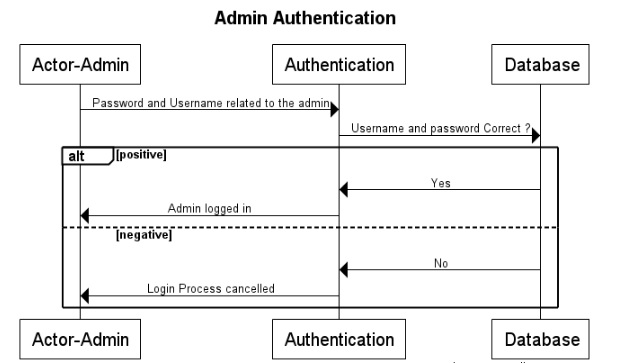
\includegraphics[width=150mm]{SequenceDiagrams/AdminAuth.jpg}
	\caption{Sequence diagram referred to "5.7 ARM: Authenticate Admin" in the requirement document. \label{6}}
\end{figure}
\begin{figure}[ht!]
	\centering
	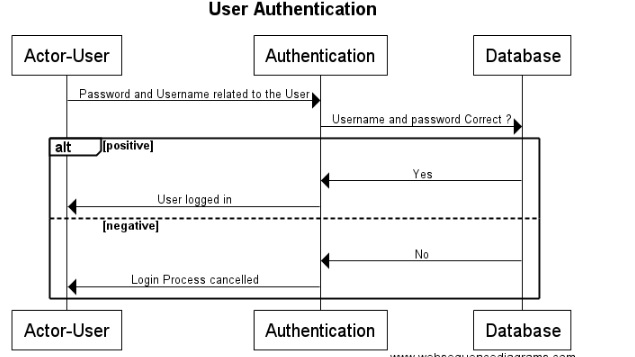
\includegraphics[width=150mm]{SequenceDiagrams/UserAuth.jpg}
	\caption{Sequence diagram referred to "5.8 URM: Authenticate User" in the requirement document. \label{7}}
\end{figure}




\end{document}
